\begin{frame}[parent={ie:agenda}, hasnext=false, hasprev=false]
	\frametitle{Avaliação de qualidade de produto}

	\begin{block:fact}{Avaliação de qualidade de produto}
		\begin{itemize}
		 \item Repetível (pelo mesmo avaliador)
		 \item Reproduzível (por outro avaliador)
		 \item Imparcial (não ser influenciada)
		 \item Objetivo (resultados devem ser factuais)
		\end{itemize}
	\end{block:fact}
\end{frame}



\begin{frame}[hasnext=true, hasprev=true]
	\frametitle{Avaliação de qualidade de produto}
	\framesubtitle{ISO 14598}

	\begin{block:concept}{ISO 14598}
		Conjunto de normas ISO/IEC sobre a avaliação de produtos de software.
	\end{block:concept}
	
	\begin{block:fact}{Partes da norma}
		\begin{itemize}
			\item ISO/IEC 14598-1: Visão geral.
			\item ISO/IEC 14598-2: Planejamento e gestão.
			\item ISO/IEC 14598-3: Processo para desenvolvedores.
			\item ISO/IEC 14598-4: Processo para adquirentes.
			\item ISO/IEC 14598-5: Processo para avaliadores.
			\item ISO/IEC 14598-6: Documentação de módulos de avaliação.
		\end{itemize}
	\end{block:fact}
	
	\note{
		ISO/IEC 14598-2 fornece requisitos, recomendações e diretrizes para uma
		função de apoio responsável pela gestão da avaliação de produto de software
		e pelas tecnologias necessárias para a avaliação de produto de software. 
	}
\end{frame}

\begin{frame}
	\frametitle{ISO 14598-1}
	\framesubtitle{Visão geral do processo de avaliação}

	\begin{block:fact}{Fases}
		\begin{itemize}
			\item Estabelecimento de requisitos de avaliação
			\item Especificação da avaliação
			\item Projeto da avaliação
			\item Execução da avaliação
		\end{itemize}
	\end{block:fact}
\end{frame}


\begin{frame}
	\frametitle{ISO 14598-1}
	\framesubtitle{Visão geral do processo de avaliação}

	\begin{block:fact}{}
		\centering
		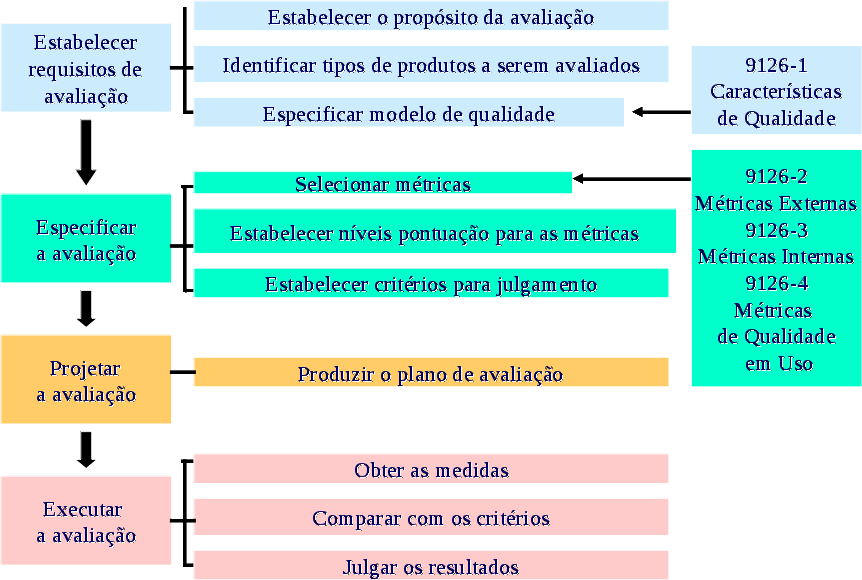
\includegraphics[width=\textwidth]{software-engineering/project-management/product/iso14598/iso14598-evaluation-process}
	\end{block:fact}
\end{frame}

%
%\begin{frame}
%	\frametitle{ISO 14598-1}
%	\framesubtitle{Requisitos de avaliação}
%
%	\begin{block:procedure}{Estabelecimento de requitos de avaliação}
%		\begin{enumerate}
%			\item Estabelecer propósito da avaliação
%			\item Identificar tipos de produtos a serem avaliados.
%			\item Especificar modelo de qualidade
%			\begin{itemize}
%				\item Por exemplo, o ISO 9126-1.
%			\end{itemize}
%		\end{enumerate}
%	\end{block:procedure}
%	
%	\note{
%		Para a fase de estabelecimento de requisitos de avaliação é necessário que 
%		tais requisitos sejam transformados em características de qualidade que
%		estão de acordo com o modelo de qualidade da ISO/IEC 9126-1. 
%		
%		Essa fase ressalta a importância dessas características  por meio da 
%		declaração do uso esperado do produto e de riscos associados.
%		
%		Dependendo do propósito da avaliação, outras normas podem ser utilizadas em
%		conjunto:
%		\begin{itemize}
%			\item ISO/IEC 14598-3: objetivo da avaliação é um produto que está sendo desenvolvido. 
%			\item ISO/IEC 14598-4: objetivo da avaliação é a compra de um produto de software no caso de processo para adquirentes
%			\item ISO/IEC 14598-5: objetivo da avaliação é a compra de um produto de software no caso de processo para avaliadores, incluindo requisitos para avaliação de terceiros.
%		\end{itemize}
%	}
%\end{frame}
%
%
%\begin{frame}
%	\frametitle{ISO 14598-1}
%	\framesubtitle{Especificação da avaliação}
%
%	\begin{block:procedure}{Especificação da avaliação}
%		\begin{enumerate}
%			\item Escolher métricas que se correlacionem com os requisitos de avaliação
%			\item Estabelecer níveis de pontuação para cada métrica
%			\item Estabelecer critérios para julgar a avaliação
%		\end{enumerate}
%	\end{block:procedure}
%	
%	\note{
%		Exemplos de métricas externas e internas apresentados na ISO/IEC 9126-2 e
%		na ISO/IEC 9126-3 podem ser aplicados nessa fase.
%	}
%\end{frame}
%
%
%\begin{frame}
%	\frametitle{ISO 14598-1}
%	\framesubtitle{Especificação da avaliação}
%
%	\begin{block:fact}{Escolha de métricas}
%		\centering
%		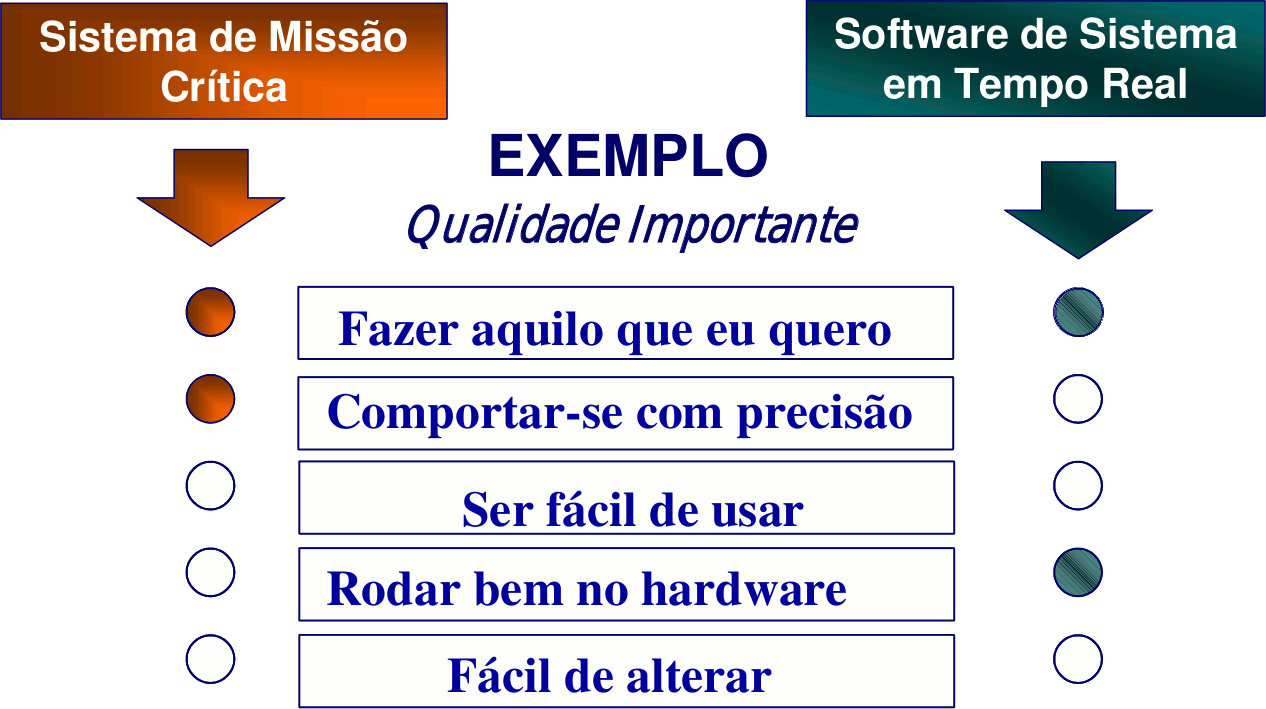
\includegraphics[width=\textwidth]{software-engineering/project-management/product/iso14598/quality-context}
%	\end{block:fact}
%\end{frame}
%
%
%
%\begin{frame}
%	\frametitle{ISO 14598-1}
%	\framesubtitle{Projeto da avaliação}
%
%	\begin{block:procedure}{Projeto da avaliação}
%		\begin{enumerate}
%			\item Documentar os procedimentos para realizar a avaliação 
%			\item Especificar os recursos necessários para executar a avaliação
%		\end{enumerate}
%	\end{block:procedure}
%	
%	\note{
%		A fase de projeto da avaliação consiste da documentação dos procedimentos
%		que serão utilizados pelo avaliador para executar a medição. 
%		
%		Os recursos necessários como, por exemplo, pessoas e técnicas, bem como a
%		sua alocação devem ser especificados para as diferentes atividades durante
%		a fase de execução da avaliação. 
%		
%		O resultado da fase de projeto da avaliação é um plano de avaliação que
%		descreve os métodos de avaliação e o cronograma das ações do avaliador. 
%	}
%\end{frame}
%
%
%\begin{frame}
%	\frametitle{ISO 14598-1}
%	\framesubtitle{Execução da avaliação}
%
%%	\begin{columns} 
%% 		\column{.4\textwidth}
%		\begin{block:procedure}{Execução da avaliação}
%			\begin{enumerate}
%				\item Coletar as medidas
%				\item Comparar com os critérios
%				\item Julgar os resultados
%			\end{enumerate}
%		\end{block:procedure}
%		
%% 		\column{.55\textwidth}
%% 		\begin{block:fact}{Escolha de métricas}
%% 			\centering
%% 			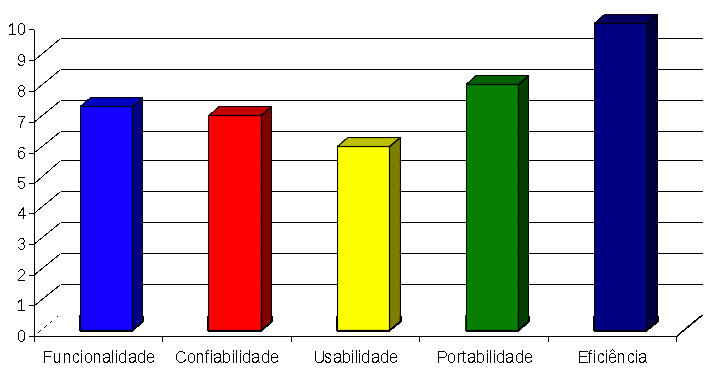
\includegraphics[width=\textwidth]{software-engineering/project-management/product/iso14598/metrics-criteria}
%% 		\end{block:fact}
%% 		\end{columns}
%		
%		\note{
%			Na fase de execução da avaliação, as métricas selecionadas são aplicadas 
%			ao produto de software, obtendo-se os valores nos níveis de pontuação. 
%			
%			Esses valores medidos são comparados com os critérios para julgamento
%			determinados anteriormente.
%		}
%\end{frame}
%
%
%
%\begin{frame}[hasnext=false, hasprev=true]
%	\frametitle{ISO 14598-1}
%	\framesubtitle{Visão geral do processo de avaliação}
%
%	\begin{block:fact}{}
%		\centering
%		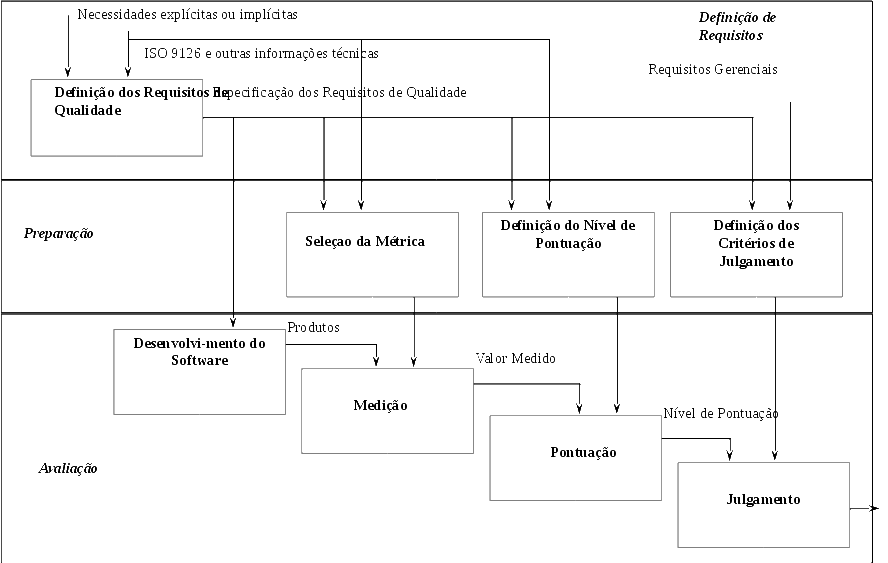
\includegraphics[width=\textwidth]{software-engineering/project-management/product/iso14598/iso14598-evaluation-process2}
%	\end{block:fact}
%\end{frame}
%
%

